\chapter{Topic Extraction Engine} \label{ch:4:topic}

The semantic analysis tool focused on 2 main text mining components in order to extract information from the news articles. This section focuses on the first of these components: the topic extraction engine, covering different data processing techniques, word and document approaches, semantic clustering and topic modelling using LDA. 

\section{Data Processing} \label{s:procesing_topic_engine}

The prepared data (from~\Cref{dataloader}) grouped by (Year, Category) comprised of a list of articles that were published in that year and assigned that category. Processing all the text for every single article would add an intensive computational burden without a huge amount of added benefit, with a potential risk of cluttering the model. For the sake of brevity, the aim was to use the article data most representative of the article. To facilitate this, a decision was made to use the titles and introduction of the articles as they contain the core information in the articles. The introduction of the article (`intro') was extracted as the first \hl{6} sentences of the article using spaCy's \texttt{SentenceSplitter}. Throughout the course of this chapter, `intro' and `article' will be used inter-changeably to represent a single news article in the corpus. 

Once the article introductions are extracted, they then undergo pre-processing before they can be vectorised for clustering. This section highlights the different pre-processing steps and key decisions made to convert the article intros into a list of tokens for the vectorisation step.

\subsection{Coreference Resolution} \label{coref}
The first step involves coreference resolution of the articles (`intros'). This involves using the pre-trained AllenNLP SpanBERT coreference resolution model for finding the set of mentions in the text that refer to the same `entity' (i.e. coreference clusters). This step was performed on the complete article intro in order for the mentions to be resolved throughout the entirety of the intro and not just on a sentence level. For example, for the text `Sean Doyle is the CEO of British Airways. Prior to this, he was the CEO of Air Lingus', if the coreference resolution was done on the sentence level, the model would miss out on resolving `he' in the second sentence to `Sean Doyle'.

\subsection{Cleaning Data} \label{data_cleaning}
Post coreference resolution of the article intros, the data needed to be `cleaned' in order to ensure that the news articles retrieved were informative and useful. This involved the following steps: 
\begin{enumerate}
    \item Removing any unnecessary characters e.g., trailing ellipsis, parenthesis etc.
    \item Removing stopwords. The spaCy model's default stopwords list was used. This significantly reduced the amount of text per article intro by removing words such as this, `that', `there', `where', `are' etc. This alone, however, was not sufficient. Given the nature of online news articles, there were some prominent phrases that showed up in several articles, e.g., \qd{Read here}, \qd{For more information}, \qd{Sourced by} etc. These were also removed as they do not provide any relevant information specific to the article, thereby reducing redundancy.

\end{enumerate}

\subsection{Named Entity Recognition}
As mentioned previously, the aim of these pre-processing steps was to obtain a \texttt{filtered\_tokens} list for each article intro which would be vectorised to represent an article as a vector for clustering. A key decision made was to remove all corresponding named entities form article intro in order to remove any dependency of the topics on these named entities. Eliminating this dependency resulted in better silhouette scores and coherence scores for semantic clustering and topic extraction as detailed in~\Cref{s:preprocess_clustering} and~\Cref{s:preprocess_topic} respectively. 

This step was done before tokenisation as named entities can often be a collection of words such as ``British Airways", ``Paul Sweeney", ``New Haven" etc. and removing these post-tokenisation would not be ideal as they would lose their semantic meaning as tokens. For instance, post tokenisation, the model would try to remove `New', `Haven' from the article intro. Therefore, regex patterns were used to remove all the occurrences of the extracted entities in an article. This included removing all entity types which included but were not limited to, `PER', `LOC', `DATE', `ORG'. This also had a performance gain over the post-tokenisation approach as it avoided the lookup for each token against the unwanted entity tokens list.

The process of extracting these entities from the article corpus using the Fine Grained NER model (refer~\Cref{s:models}) and the BILOU encoding scheme for NER is detailed in~\Cref{alg:named_ents}.

\begin{tabularx}{\textwidth}{X X X X X} 
  \textbf{B} & \textbf{I}  & \textbf{L}  & \textbf{O}  & \textbf{U} \\
  beginning & inside & last & outside &  unit \\
  \end{tabularx}

The output from the NER model gives a set of words and their corresponding entity tags. In essence, the algorithm shows the process of joining the entity tokens to build the entity phrases starting from the `beginning' token until the `last' token. Words with `Outside' as a tag mean that the word is not an entity while `unit' refers to single word entities.  

\begin{algorithm}[H]
  \caption{Extract Named Entities}
  \label{alg:named_ents}
  \begin{algorithmic}   
  \State $entities \leftarrow empty \ set$
  \State $words, tags \leftarrow \text{ner\_model.predict}(sentence)$
  \ForAll{$word, \ tag$ $\in$ zip($words, tags$) } 
    \If{t == `O'}  \State {continue}  \EndIf
    \State $ ent\_position, ent\_type$ = tag.split(`--')
    \If{t == `U'} 
    \State{$entities$.add($word$)}
    \Else
      \If{ $ent\_position$ == `B'} 
      \State $ent := word$
      \ElsIf { $ent\_position$ == `I'} 
      \State  $ent := ent + word$
      \ElsIf { $ent\_position$ == `L'} 
      \State  $ent := ent + word$
      \State{$entities$.add($ent$)}
      \EndIf
    \EndIf
  \EndFor
\end{algorithmic}
\end{algorithm}

\subsection{Filtering Tokenised Data} \label{filtered_tokens}
Once the data was cleaned and void of the pre-determined entity types, the article intros were tokenised and normalised. This was done using the spaCy library's \texttt{Tokeniser} and \texttt{Lemmatiser} pre-trained on the English language model: \hl{en\_core\_web\_lg} (refer to~\Cref{libraries}). Normalisation was done through lemmatisation (to obtain the base forms of the tokens). This was chosen instead of stemming as it guaranteed more semantically meaningful tokens which for reasons detailed in~\Cref{normalisation}. The process of obtaining a list of tokens for each article intro was as follows:
\begin{enumerate}
    \item Each sentence in the intro was turned into a list of tokens.
    \item These tokens were filtered by their Part-Of-Speech (POS) tags against the allowed POS tags, which was restricted to nouns (`NOUN').
    \item Tokens that were numeric and less than 2 characters were also removed. 
    \item The remaining tokens were lemmatised and added to the \texttt{filtered\_tokens} list for the given article.
\end{enumerate}

It is important to note that the allowed POS tags were originally set to include nouns (NOUN), adjectives (ADJ), verbs (VERB) and adverbs (ADV). This resulted in a lot of unnecessary tokens such as `because', ‘did’, ‘very’ etc. Different combinations of the allowed POS tags were experimented with, ultimately allowing only nouns to comprise the \texttt{filtered\_tokens} for each article (`intro'). This decision was primarily based on the resulting clustering scores when the allowed POS tags were limited to `NOUN' and when they included `NOUN', `ADJ', `VERB' and `ADV' as discussed in the evaluation in~\Cref{s:pos_clustering}.

\section{Semantic Clustering} \label{s:semantic_clustering}

The first step to generating semantic clusters of articles is to get the corresponding article vectors. This involves vectorising the individual tokens in \texttt{filtered\_tokens} list for each article intro.

\subsection{Word embedding approaches} \label{word_embed_approaches}
To vectorise the tokens, different pre-trained word embedding models were used. These approaches (in chronological order) with their strengths and shortcomings are outlined below.

\renewcommand\arraystretch{2}
\captionsetup{singlelinecheck=false, labelfont=sc, labelsep=quad}
\begin{longtable}{@{\,}r <{\hskip 2pt} !{\foo} >{\arraybackslash}p{14cm}}
\centering

TF-IDF & Term frequency-inverse document frequency is a statistical metric that examines the comparative relevance of a word/token with respect to an article intro in the collection of articles. Representing the tokens as their TF-IDF measure first involves calculating the term frequency (TF) using the bag of words (BoW) approach from Gensim \texttt{Doc2BoW}. To account for overlapping terms across all article intros, the term frequency was multiplied by the inverse document frequency to weigh down the terms whose high frequency is not unique to a document (Refer to  \hl{Add in BCKG}). A dense document-term using the TF-IDF values for each term is used to represent the article intro as a vector for clustering. \\

Word2Vec & The next approach saw the use of Google's \texttt{Word2Vec} model (from Gensim) to obtain pre-trained word embeddings for each token in an article's corresponding \texttt{filtered\_tokens} list. The issue with the previous approach was that it represented the statistical information about a document, in particular, the measure of the frequency of words in a document, rather than any semantic information about a document. \texttt{Word2Vec} embeddings, on the other hand, return a vector for each word that accounts for semantic similarity (based on cosine distance) between the words represented by the vectors~\cite{word2vec}. \\

GloVe & The final approach was to use Stanford's \texttt{GloVe} (global vector) embeddings from Gensim. \texttt{GloVe} as been pre-trained on Wikipedia and Gigaword 5, consisting of a vocabulary of 400,000 words which are represented by 300 dimensional vectors~\cite{glove}. The advantage of this approach over previous approaches is that it makes use of global statistics such as word co-occurrences to obtain word vectors. Using these embeddings also saw an improvement in the silhouette scores when deriving the semantic clustering of articles as detailed in~\Cref{s:word_embeddings}. \\
\end{longtable}

\newpage
\subsection{Document embeddings}

In~\Cref{filtered_tokens}, \texttt{filtered\_tokens} are defined as the all \textit{relevant} tokens for each article intro. As mentioned above, the filtered tokens were vectorised using the \texttt{GloVe} embeddings~\cite{glove} resulting in a list of vectors corresponding to the \texttt{filtered\_tokens}. In order to get the document vectors from these word vectors, two approaches were tested: 

\renewcommand\arraystretch{2}
\captionsetup{singlelinecheck=false, labelfont=sc, labelsep=quad}
\begin{longtable}{@{\,}r <{\hskip 2pt} !{\foo} >{\arraybackslash}p{14cm}}
\centering

Approach 1 & The corresponding tokens in \texttt{filtered\_tokens} list for the article intro are vectorised (using \texttt{GloVe} embeddings) and averaged to find the corresponding article vector. This was a simple approach that gave equal importance to each token associated with the article intro. \\

Approach 2 & Rather than simply averaging the token vectors for each article intro, the document vector was calculated using a weighted sum of corresponding word vectors (from \texttt{filtered\_tokens}). This was done by using a TF-TDF model to get the term-frequency inverse document frequency weight for each token in the corresponding article. This meant that words that appeared in high frequency unique to the associated article contributed more to the document vector than those with a lower frequency or those that appeared frequently in other article intros. \\

Approach 3 & Building on the previous approach, this method selects the top 10 most representative words based on the TF-IDF weightings and performs the weighted average to generate the article vector.\\
\end{longtable}
\vspace{-2ex}
\begin{figure}[H]
  \centering
  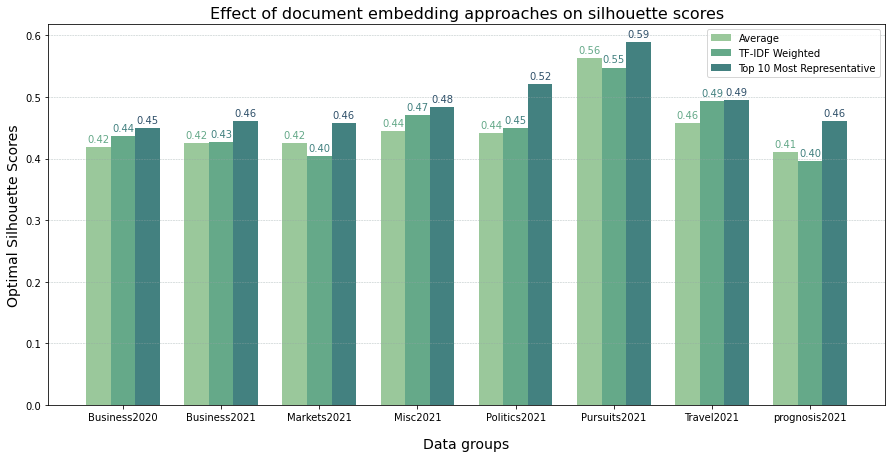
\includegraphics[width=0.8\linewidth]{images/eval/doc_embedding_sil.png}
  \vspace{-1em}
  \caption{Effect of document vector generation approaches on clustering silhouette scores}
  \label{fig:doc_embeddings}
  \end{figure}

  \vspace{-1em}
\Cref{fig:doc_embeddings} shows how the different word embeddings approaches effect the `goodness' of clustering indicated by silhouette scores. The consensus derived is that Approach 3, which describes calculating the article (document) vector by computing the weighted average of the top 10 most relevant words (using the TF-IDF metric), performs better than the other 2 approaches mentioned. Approach 3 results in a 9.36\% improvement in silhouette score compared to Approach 1 (simple averaging of word vectors) and an 8.37\% improvement compared to Approach 2 (weighted (TF-IDF) average of all word vectors). This led to the decision of using Approach 3 as the method for document vector generation.
%  \hl{Figure out how to add the silhouette score stuff before?}

%%%%%%%%%%%%%%%%%%%%%%%%%%%%%%%%%%%%%%%%%%%%%%%%%%%%%%%%%%%%


\subsection{Dimensionality Reduction}

\subsubsection{Normalising Data}
The first step is to normalise the article vectors in order to eliminate redundancy in data and standardise the features (components of the vector) in case of high variance, which contributes to better clustering. Additionally, when it comes to performing principal component analysis for the article vectors, the vector components (features) should be independent of their standard deviation or variance to get a good covariance matrix among the features.  

\subsubsection{Principal Component Analysis}

As established previously (refer to~\Cref{word_embed_approaches}), \texttt{GloVe} document embeddings result in a 300-dimensional vector. Clustering the document vectors becomes inefficient and meaningless at these high dimensions as the concept of distance becomes less precise as the number of dimensions increases~\cite{pca_clustering} as the volume of space increases exponentially making the available data spare - curse of dimensionality. For any given point in this high n-dimensional space, the difference in 'distance' (euclidean) to the closest point $d_min$ and the farthest point $d_max$ with respect to the $d_min$ becomes negligible~\cite{nearest_neighbour}. 

\[ \lim_{n\to\infty} \frac{d_{max} - d_{min}}{d_{min}} \to0\]

\vspace{-2ex}
\begin{figure}[H]
  \centering
    \begin{minipage}[t]{.49\textwidth}
      \centering
      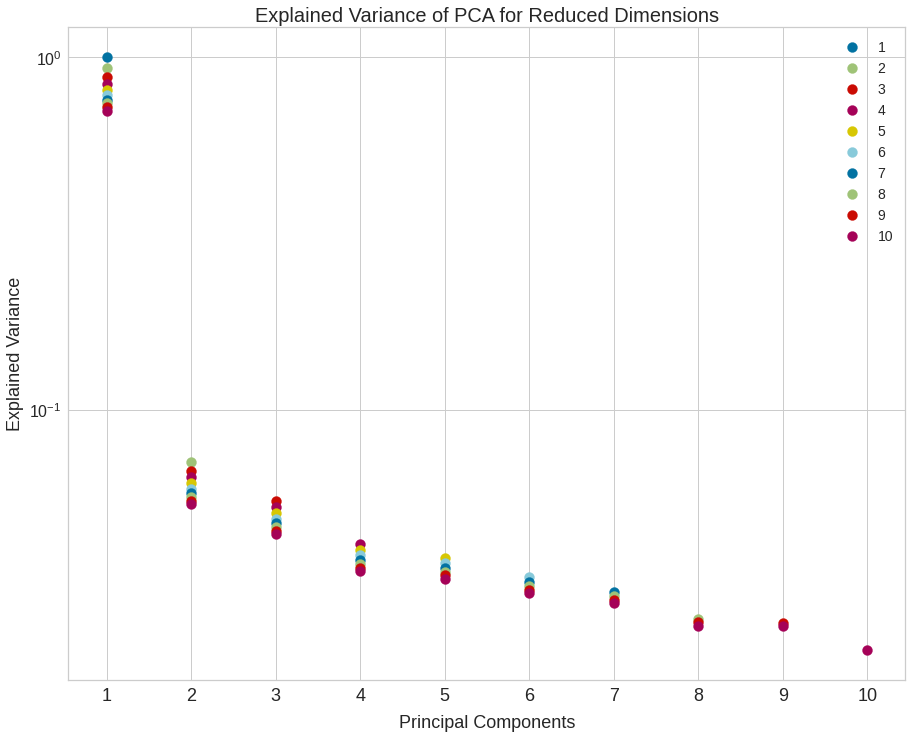
\includegraphics[width=\textwidth]{images/eval/explained_variances.png}
      \caption{-}
      \label{fig:explained_variance}
    \end{minipage}
    \begin{minipage}[t]{.49\textwidth}
      \centering
      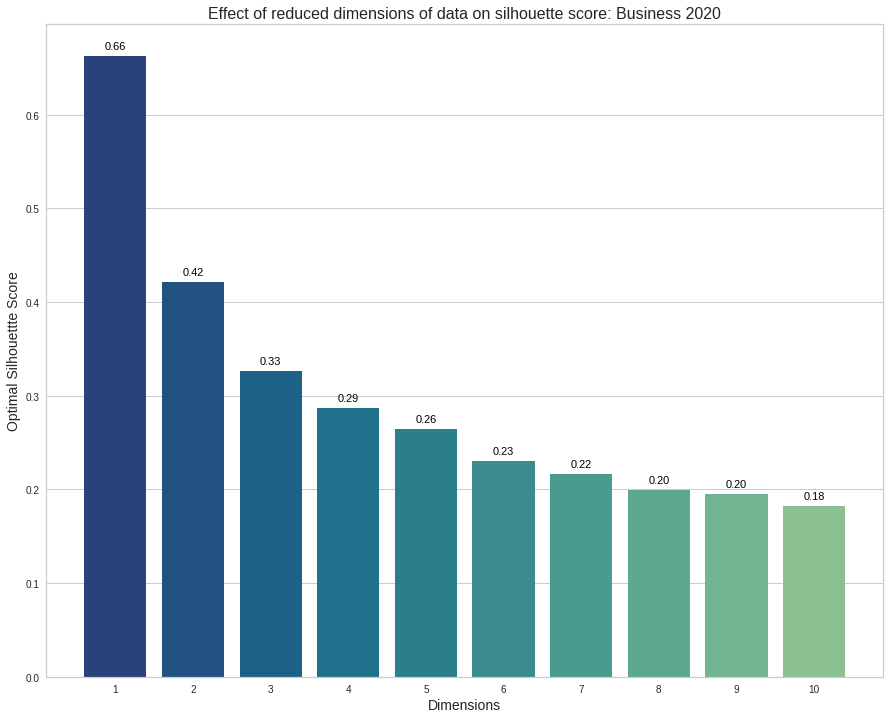
\includegraphics[width=\textwidth]{images/eval/pca_silhouette.png}
      \caption{-}
      \label{fig:pca_sil}
    \end{minipage}
  \end{figure}

  The concept of clustering these articles relies on grouping similar articles together based on their attributes. The similarity is determined based on the vectorised \texttt{filtered\_tokens}. However, given the high dimensional data, some of these attributes will not be relevant in determining the clusters. The goal is to find the attributes (vector components) with the most variance across the documents vectors to represent the features. This is accomplished by performing principal component analysis (PCA) on the normalised high-dimensional input vector space to map to a lower dimensional space, whilst minimising information loss~\cite{pca_clustering}.

  As seen in~\Cref{fig:explained_variance}, when the article vector space is projected to dimension=1, the variance is explained entirely by dimension 1 (blue dot). As the number of dimensions increase, the number of principal components increase, the main proportion of the variance can still be explained by the first principal components (close to 1). For instance, projecting to dimension=10, the explained variances for each of the 10 principal components is as follows: 
  \begin{table}[H]
      \centering
  \renewcommand{\arraystretch}{1.1}
  \begin{tabularx}{\textwidth}{|X|X X X X X X X X X X|} 
    \hline
    PC & \textbf{1} & \textbf{2}  & \textbf{3}  & \textbf{4}  & \textbf{5} & \textbf{6} & \textbf{7}  & \textbf{8}  & \textbf{9}  & \textbf{10}\\
    \hline
    EV & 0.88 & 0.026 & 0.021 & 0.014 & 0.011 & 0.010 & 0.0094 & 0.0090 & 0.0082 & 0.0074\\ 
    \hline
    \end{tabularx}
  \end{table}
  
  Therefore, 88\% of the variance (EV) can be explained by the first principal component (PC) alone and so the article vector space can be transformed using PCA with dimensions=1.~\Cref{fig:pca_sil} shows the effect of transforming the article vector space to different dimensions on the silhouette scores, which represent the `goodness of clustering'. It indicates that transforming the vectors to a single dimension (using PCA) result in the highest silhouette score. Therefore,~\Crefrange{fig:explained_variance}{fig:pca_sil} conclude that the setting the dimension to 1 for PCA transformation results in the most optimal clustering whilst retaining majority of the information (variance).

\subsection{KMeans Clustering}
Once the normalised data is mapped to the lower subspace, the articles are clustered based on their cosine similarity~\cref{eq:cosine_sim} using cosine distance as the distance function~\cref{eq:cosine_distance} and KMeans as the clustering technique. This was done using the \texttt{sklearn} library's \texttt{kmeans} function with `euclidean distance'~\cref{eq:euc_distance} as distance metric. This is feasible given the linear relationship between Euclidean distance and  cosine distance~\cite{kmeans} for normalised vectors shown in~\cref{eq:relationship_ce}.

\begin{align}
  \mathit{For \ normalised \ vectors,} \ x, y:  \sum x_i^2 &= 1,  \sum y_i^2 = 1 \label[equationX]{eq:normalised} &\\ 
  \mathit{Cosine \ Similarity,} \ cos(x, y) &= \frac{\sum x_i y_i}{\sqrt{\sum x_i^2 y_i^2}}  \nonumber &\\ 
   &= \sum x_i y_i \label[equationX]{eq:cosine_sim} &\\
   \mathit{Cosine \ Distance} &= 1 - cos(x, y) \label[equationX]{eq:cosine_distance} &\\
   \mathit{Euclidean \ Distance,} \ || x - y ||_2^2  &= \sum (x_i -  y_i)^2  \label[equationX]{eq:euc_distance} &\\
                 &= \sum (x_i^2 + y_i^2 - 2 x_i y_i)  \nonumber &\\
                 &= \sum x_i^2 + \sum y_i^2 - 2\sum x_i y_i   \nonumber &\\
                 &= 1 + 1 - 2 cos(x, y)  \nonumber &\\
                 &= 2 (1 - cos(x, y))  &\\
                 &= 2 (\mathit{Cosine \ Distance}) \label[equationX]{eq:relationship_ce}
\end{align}


% \todonum[inline, color=darkgray]{Add kmeans formula - MDS?}

Furthermore, to avoid falling into the trap of random centroids initialization, a major shortcoming of the KMeans method, the clustering was done with KMeans++. KMeans++ offers a better initialisation approach for centroids, in which the first one is picked at random and the subsequent centroids are chosen with a probability proportional to the squared distance from the closest chosen centroid.


\subsection*{Determining the optimal number of clusters}
Determining the number of clusters (k) in KMeans is a crucial factor to consider. This was done by computing the KMeans clustering algorithm for different values of k varying from 2 (minimum number of clusters) to m (maximum number of clusters), and picking the optimal k based on a comparing statistic. The two comparison statistics considered were: Elbow method with Within Cluster Sum of Square distance (WCSS) and Silhouette score. 

\subsubsection{Method 1: Minimising WCSS using Elbow Method}
The elbow method uses the distance (Euclidean) between the cluster centroid and its members, i.e., intra-cluster variance (distortion score or WCSS) to determine how many clusters are needed to encapsulate the variance of the data. In particular, it minimises the loss function: WCSS (a.k.a. distortion score) which is the sum of the squared distance between each point and the centroid in a cluster~\cite{elbowvssil}.
\vspace{-1ex}
\begin{align}
  \mathit{WCSS} &=  \sum^{C_n}_{C_k} (\sum^{d_m}_{d_i \in C_i} || d_i - C_k ||_2^2) \label{eq:wcss}
\end{align}

As seen in~\Cref{fig:elbow}, the elbow (bend) in the plot determines the optimal number of clusters, i.e., the k value = 4. The main drawback of using the lowest distortion score to determine the optimal number of clusters is that as long as the number of clusters (k) increases, the distortion score (WCSS) will decrease because the points will be closer to their centroids. Hence, the elbow (bend) is used to determine the minimum number of clusters with a reasonably low distortion score as seen in~\Cref{fig:elbow}, which gives the optimal number of clusters, k=4.

\begin{figure}[H]
\centering
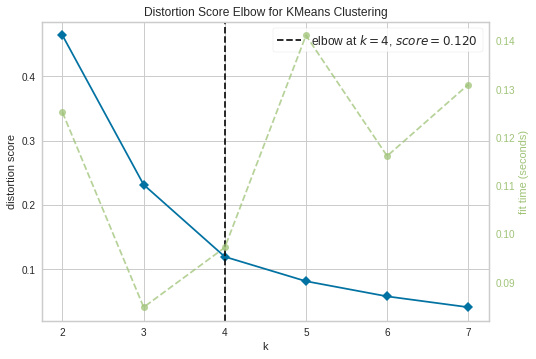
\includegraphics[scale=0.4]{images/elbow.png}
\caption{`Business 2020' Elbow Method Plot for k=2..7}
\label{fig:elbow}
\end{figure}

\subsubsection{Method 2: Silhouette score}

The second approach involved using the silhouette score. Unlike, the elbow method silhouette score accounts for both how close a point is within its cluster (cohesion)~\cite{elbowvssil} and other clusters (separation)~\cite{silhouette}.

\begin{center}
    $\mathit{Silhouette \ Score }= \mathit{mean}_i (\frac{S_i - C_i}{\max(S_i, C_i)}) $
\end{center}
% \ mathrm
where 
cohesion, $C_i$ = average distance between i and all points within its cluster.
separation, $S_i$ = average distance between i and all points not in its cluster.

The silhouette score is the mean of Sil(i) for all points i in the data. It ranges from -1 to 1. A value closer to 1 indicates that clusters are well separated and distinguished. A value ~ 0 indicates significant overlapping between the clusters, and the clusters are not distinguished. A value near -1 indicates that clusters are assigned incorrectly.

\begin{figure}[H]
\centering
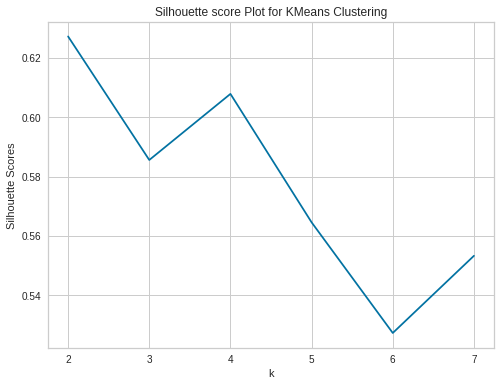
\includegraphics[width=0.4\linewidth]{images/sil_kmeans_.png}
\caption{`Business 2020' Silhouette Plot for KMeans clustering with k=2..7}
\label{fig:sil_kmeans}
\end{figure}
\vspace{-2ex}

\begin{figure}[H]
\begin{minipage}{0.45\linewidth}
\centering
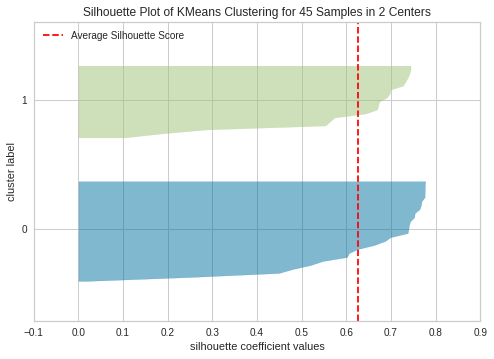
\includegraphics[width=\linewidth]{images/cluster 2.png}
\caption{`Business 2020' Silhouette Diagram: score = 0.627 for k=2}
\label{fig:cluster2}
\end{minipage}
\hfill
\begin{minipage}{0.45\linewidth}
\centering
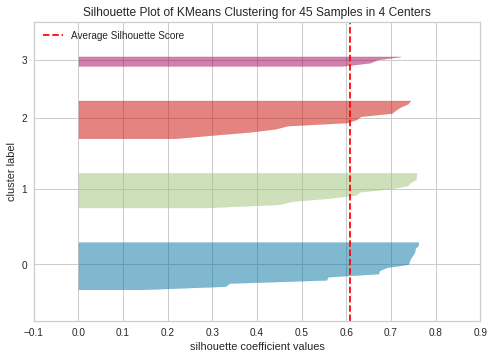
\includegraphics[width=\linewidth]{images/cluster 4.png}
\caption{`Business 2020' Silhouette Diagram: score = 0.607 for k=4}
\label{fig:cluster4}
\end{minipage}
\end{figure}

\vspace{-1ex}
From~\Cref{fig:sil_kmeans}, it is apparent that while selecting k=4 (as found by Elbow Method in~\Cref{fig:elbow}) results in a good clustering, a better clustering can be achieved by selecting k=2, as it gives a higher silhouette score, suggesting less overlap. \Crefrange{fig:cluster2}{fig:cluster4} show the silhouette diagram for number of clusters, k=2 and k=4 respectively. The cluster thickness denotes the size of the cluster, while the width represents the sorted silhouette coefficients of instances in the cluster. Observing~\Cref{fig:cluster2} (k=2) reveals that both clusters are roughly equal in size, whereas~\Cref{fig:cluster4} (k=4), illustrates a higher disparity in size as Cluster 3 is less than half the size of others. This is indicative of some clusters being split, thereby resulting in a suboptimal silhouette score. 

Out of the two approaches, the decision was made to go with the silhouette score as it factors both how compact a cluster is and how distinct it is. This is a vital consideration given that the aim of the engine is to distinctly cluster the news articles with minimal overlap, in order to minimise common topics within clusters post topic modelling (performed on each cluster). 

\subsection*{Find n most representative docs} \label{sec:Find_n_docs}

Once the articles are clustered, the goal is to obtain a cluster-to-article mapping. However, given the high volume of data, it is not as necessary to consider every single article in the cluster particularly those that are not close to their respective cluster centroids. A pre-determined value $n_{max}$ is selected, and the euclidean distance from each member (article) to its centroid is computed. The articles are sorted in increasing order of distance and the top n articles are selected for each cluster. Furthermore, since the next step in the topic extraction engine entails modelling topics on these semantic clusters, it is futile to consider the sparse clusters that have very few (less than $n_{min}$) members as they will not spawn any good topics and are therefore omitted. These values $n_{max}$ and $n_{max}$ are calculated based on the mean and standard deviation of the sizes of semantic clusters obtained as shown in~\crefrange{eq:nmin}{eq:nmax}.
\vspace{-1px}
\begin{align}
  n_{min} &= \lfloor mean(|C_1|, |C_2|, ..., |C_n|) - std(|C_1|, |C_2|, ..., |C_n|) \rfloor \label[equationX]{eq:nmin} &\\
  n_{max} &= \lceil mean(|C_1|, |C_2|, ..., |C_n|) + std(|C_1|, |C_2|, ..., |C_n|) \rceil \label[equationX]{eq:nmax}
\end{align}

\section{Topic Modelling}

Post semantic clustering, the aim is to extract topics associated with each cluster. This was done through topic modelling, which follows an unsupervised approach of extracting the top topics from a corpus. In particular, the model used was the Latent Dirichlet allocation (LDA) from the Gensim library. 

As explained in~\Cref{Topic Modelling appoaches}, each document (article intro) is made up of several words (\texttt{filtered\_tokens}) and each topic has several (key)words associated with it. Given that the LDA model is a probabilistic model, it tries to estimate the topic distribution for each article as well as the word distribution for each topic. The motivation for using LDA is to get the topic-document probability distribution which can then be used to get the topics associated with a document. For the scope of this problem, this was limited to one dominant topic. 

It is important to note that topic modelling LDA does not rely on semantic information, this is why the decision was made to obtain semantic clusters first and then model topics on them.
\vspace{-1ex}
\subsection{Corpus Decisions}

From the data processing steps detailed in~\Cref{s:procesing_topic_engine}, the article intros have already been cleaned, lemmatised, filtered and tokenised to get their corresponding \texttt{filtered\_tokens}, which are void of any stopwords and named entities and only contain nouns. For the input corpus passed to the LDA, there were certain key decisions made, which were influenced by previous studies and quantitive evaluation (discussed in \Cref{s:evaluation_topic_extraction}). Using the \texttt{filtered\_tokens} satisfied most of these requirements which are explained below: 

\begin{enumerate}
  \item \textbf{Noun-only corpus}: Based on previous studies~\cite{nouns_only_lda}~\cite{efficient_noun_only_approach}, and the results from~\Cref{s:pos_topic} which saw improved coherence values of topics averaged across clusters and \hl{fewer numbers of `unpopular' topics (i.e. those with few associated articles)}, the decision was made to limit input corpus to nouns (satisfied by \texttt{filtered\_tokens}). This aligned with the intuition that nouns are better indicators of a topic as they provide more semantic context. Opening the corpus to other POS categories, for instance, ADJ, VERB (Appendix~\Cref{appendix:pos}), will result in sub-optimal topics since the LDA model will give "fast" and "pandemic" equal importance.
  
  \item \textbf{No Named Entities}: Similar to semantic clustering, the decision as made to omit all named entities from the LDA corpus. This was also satisfied by the \texttt{filtered\_tokens} where the entities found using the Fine-Grained NER model were removed. As seen in ~\Cref{fig:pos_topic}, omitting named entities improved the coherence score of the topics. 

  \item \textbf{Using Bigrams}: Inspired by \cite[`Beyond bag of words']{bigrams_lda}, a decision made was to augment the corpus using n-grams, in particular, bigrams, rather than solely using unigrams. This allowed the model to consider a combination of two commonly occurring words across documents, e.g., “coronavirus\_pandemic”, “aviation\_industry” etc. This was particularly relevant given the dataset of news articles containing common `noun chunks' which can be used to infer topics. The bigrams are derived using Gensim's \texttt{Phraser} which uses colocation detection, and are appended to \texttt{‘filtered\_tokens’.}
  
  \item \textbf{TF-IDF}: In LDA, the document need to be transformed into numeric feature vectors which form the corpus. Since it does not rely on the article's semantic information and builds topic estimators based on words, article and topics, it uses frequency vectors as obtained by Bag-of-Words and Term Frequency-Inverse Document Frequency. The decision was made to use TF-IDF over the more common Bag-of-Words~\cite{topic_models}, in an attempt to minimise overlap of topics as each article will be associated with one dominant topic.
\end{enumerate}

% \subsection{Implementation}
% \todonum[inline]{Pseudocode/ Diagram?}
% \begin{enumerate}
%     \item \textbf{Bigrams:} Using Gensim’s Phraser model which uses colocation detection, the bigrams are generated (a\_b where a and b are nouns), which are appended to the ‘filtered\_tokens’.
%     \item \textbf{Corpus:} Based on the decisions highlighted in section ???, the corpus is defined as a collection of filtered, tokenised, lemmatised nouns and noun-chunks (bigrams) of article intros, barring entities and stopwords.
    
%     % <Potentially talk about PMI scoring - PMI-like scoring as described in Mikolov, et. al: “Distributed Representations of Words and Phrases and their Compositionality”.>
    
%     \item \textbf{Dictionary:} A dictionary mapping the words in the corpus to their integer ids is created using the Dictionary \hl{wrapper?} in Gensim. 
%     \item \textbf{BoW, TF-IDF:} The corpus is passed to the bag of words model from Gensim and then is transformed by the TF-IDF to return a weighted frequency of words in article intros. This is the input to the LDA model. 
% \end{enumerate}

% Pseudocode: 
% For each cluster, 
% 	Get articles indexes in the clusters. 
% 	Get the corresponding filtered tokens (ones that were used to vectorise the article in clustering) => dictionary 
% 	Make n grams 

\subsection{Determining number of latent topics}

A key contributor in determining the quality of the topics extracted is tuning the {num\_topics} parameter \texttt which represents number of topics outputted by the LDA. A low value will result in too few or overly generalised topics whereas a high value results in uninterpretable topics that ideally should have been merged~\cite{topic_score}. Previous studies~\cite{cv_abstract}~\cite{cv_space} show that one of the best methods to determine the number of latent topics is to measure CV coherence, which has a high correlation with human judgments of topic interpretability. This metric computes the normalised pointwise mutual information (NPMI) and cosine similarity of content vectors of words, derived based on their co-occurrences~\cite{cv_space}.

This was achieved by using \texttt{CoherenceModel} with the `c\_v' setting from the Gensim library. The optimal number of topics (i.e., value resulting in the highest coherence score) is computed for each cluster by running the LDA model with different values of k varying from min\_topics (defaulted to 2) to max\_topics (dependent on the size of cluster), and the LDA model with the highest resulting coherence is chosen. The motivation for bounding the max\_topics was to ensure topics would have at least the minimum number of article intros (=2). Additionally, pruning the number of LDA runs had performance gain.

\subsubsection*{Dominant Topic-Article Mapping} \label{sec:topic_article_mapping}
Once the optimal value of n\_topics is determined, the corresponding LDA model is applied to the TF-IDF corpus to get the resulting article-topic distribution. This returns the most probabilistic topics for each article intro. This is of the form \texttt{articleId: (topicId, probability)}, where \texttt{probability} refers to the likelihood that the article belongs to the topic corresponding to the \texttt{topicId}. Of these, the most dominant topic (the highest likelihood of belonging to the topic) is selected, resulting in an 1-1 topic-article mapping. 

\vspace{-1ex}
\subsection*{Topic Name Inference}

An augmented feature of the Topic Modelling Engine was to infer the topic names from the keywords of the topic. \Cref{alg:topic_name} details the process of inferring topic names from the corresponding topic keywords. This involves splitting any bigram keywords to obtain a set of keyword tokens which are checked to ensure they are nouns, not a stopword and have an associated \texttt{Glove} vector. Using the \texttt{glove\_model.most\_similar()} method from Gensim, which computes the cosine similarity between an average of projection of resulting keyword vectors (\texttt{validKws}), the candidate topic names are obtained. These are again checked for validity in terms of whether they are a noun and are not augmented stopwords. The top 2 most similar topic name tokens that meet the validity checks are selected as the topic name for the given topic. 

\begin{algorithm}[H]
  \caption{Infer Topic Name}
  \label{alg:topic_name}
  \begin{algorithmic}   
    \Function{GetValidKeywords}{$topicKeywords$, $stopwords$, $allowed\_pos=[`NOUN']$}
    \State $validKws \gets \emptyset$
    \ForAll{$topicKw \in topicKeywords$} 
    \State $kw \gets topicKw.lemma$
    \If {$kw \in stopwords$ \AND $kw \notin GloVe.vocab$ \AND $kw.pos \notin allowed\_pos$}
    \State $continue$
    \EndIf
    \State $validKws.append(kw)$
    \EndFor
    \State \Return $validKws$
  \EndFunction

\vspace{1em}
  \Function{GetTopicName}{$topicKeywords$, $stopwords$}
    \State $kws \gets$ \Call{GetKeywordTokens}{$topicKeywords$}
    \Comment{$splits \ bigrams$}
    \State $validKws \gets$ \Call{GetValidKeywords}{$kws, stopwords$}[:5]
    \State $topicNameCands := \text{GloVe}.most\_similar(validKws, topn=5)$
    \State $validTopicNames \gets$ \Call{GetValidKeywords}{$topicNameCands, stopwords$}
    \If {$len(validTopicNames) == 0$}
    \State \Return $validKws[0]$
    \Else
    \State \Return $validTopicNames[0:2]$
    \EndIf
  \EndFunction
\end{algorithmic}
\end{algorithm}
\vspace{-1ex}
\subsection*{Topic Sentiment}
\vspace{-1ex}
\begin{algorithm}[H]
  \caption{Computing Topic Sentiment}
  \label{alg:topic_sent}
  \begin{algorithmic}   
  \Function{GetTopicSentiment}{$topicArticles$}
    \State $sentiments \gets  \emptyset$
    \ForAll {$article \in topicArticles$}
    \State $sentiments.append(roBERTa\_model.predict(article.title))$ \Comment{0: N, 1:P}
    \EndFor
    \State $avgSent = average(sentiments)$
    \If {$avgSent >= 0.4 \AND avgSent <= 0.6$}
    \State \Return `Neutral'
    \ElsIf {$avgSent > 0.6$}  \Return `Positive'
    \Else  \Return `Negative'\EndIf
  \EndFunction
\end{algorithmic}
\end{algorithm}
\vspace{-1.5ex}
The last component of the Topic Modelling Engine involves sentiment analysis. In order to compute the topic sentiment, the sentiment of each article associated with the topic is computed. For this, the RoBERTa Sentiment Treebank model is used on the article title as it serves as good descriptor of the tone of article. The model outputs a binary label, where 0 indicates `negative' sentiment and 1 indicates `positive' sentiment. These are then averaged to get the sentiment of the topic. Based on the range of this value it is assigned one of the following: 'Positive', 'Negative' and 'Neutral' as shown in~\Cref{alg:topic_sent}.

\vspace{-1ex}
\section{Results and Discussion}

This section focuses on the qualitative analysis of the results obtained from the Topic Extraction Engine displayed by the visualisation tool. 
\vspace{-2ex}
\begin{figure}[H]
  \centering
  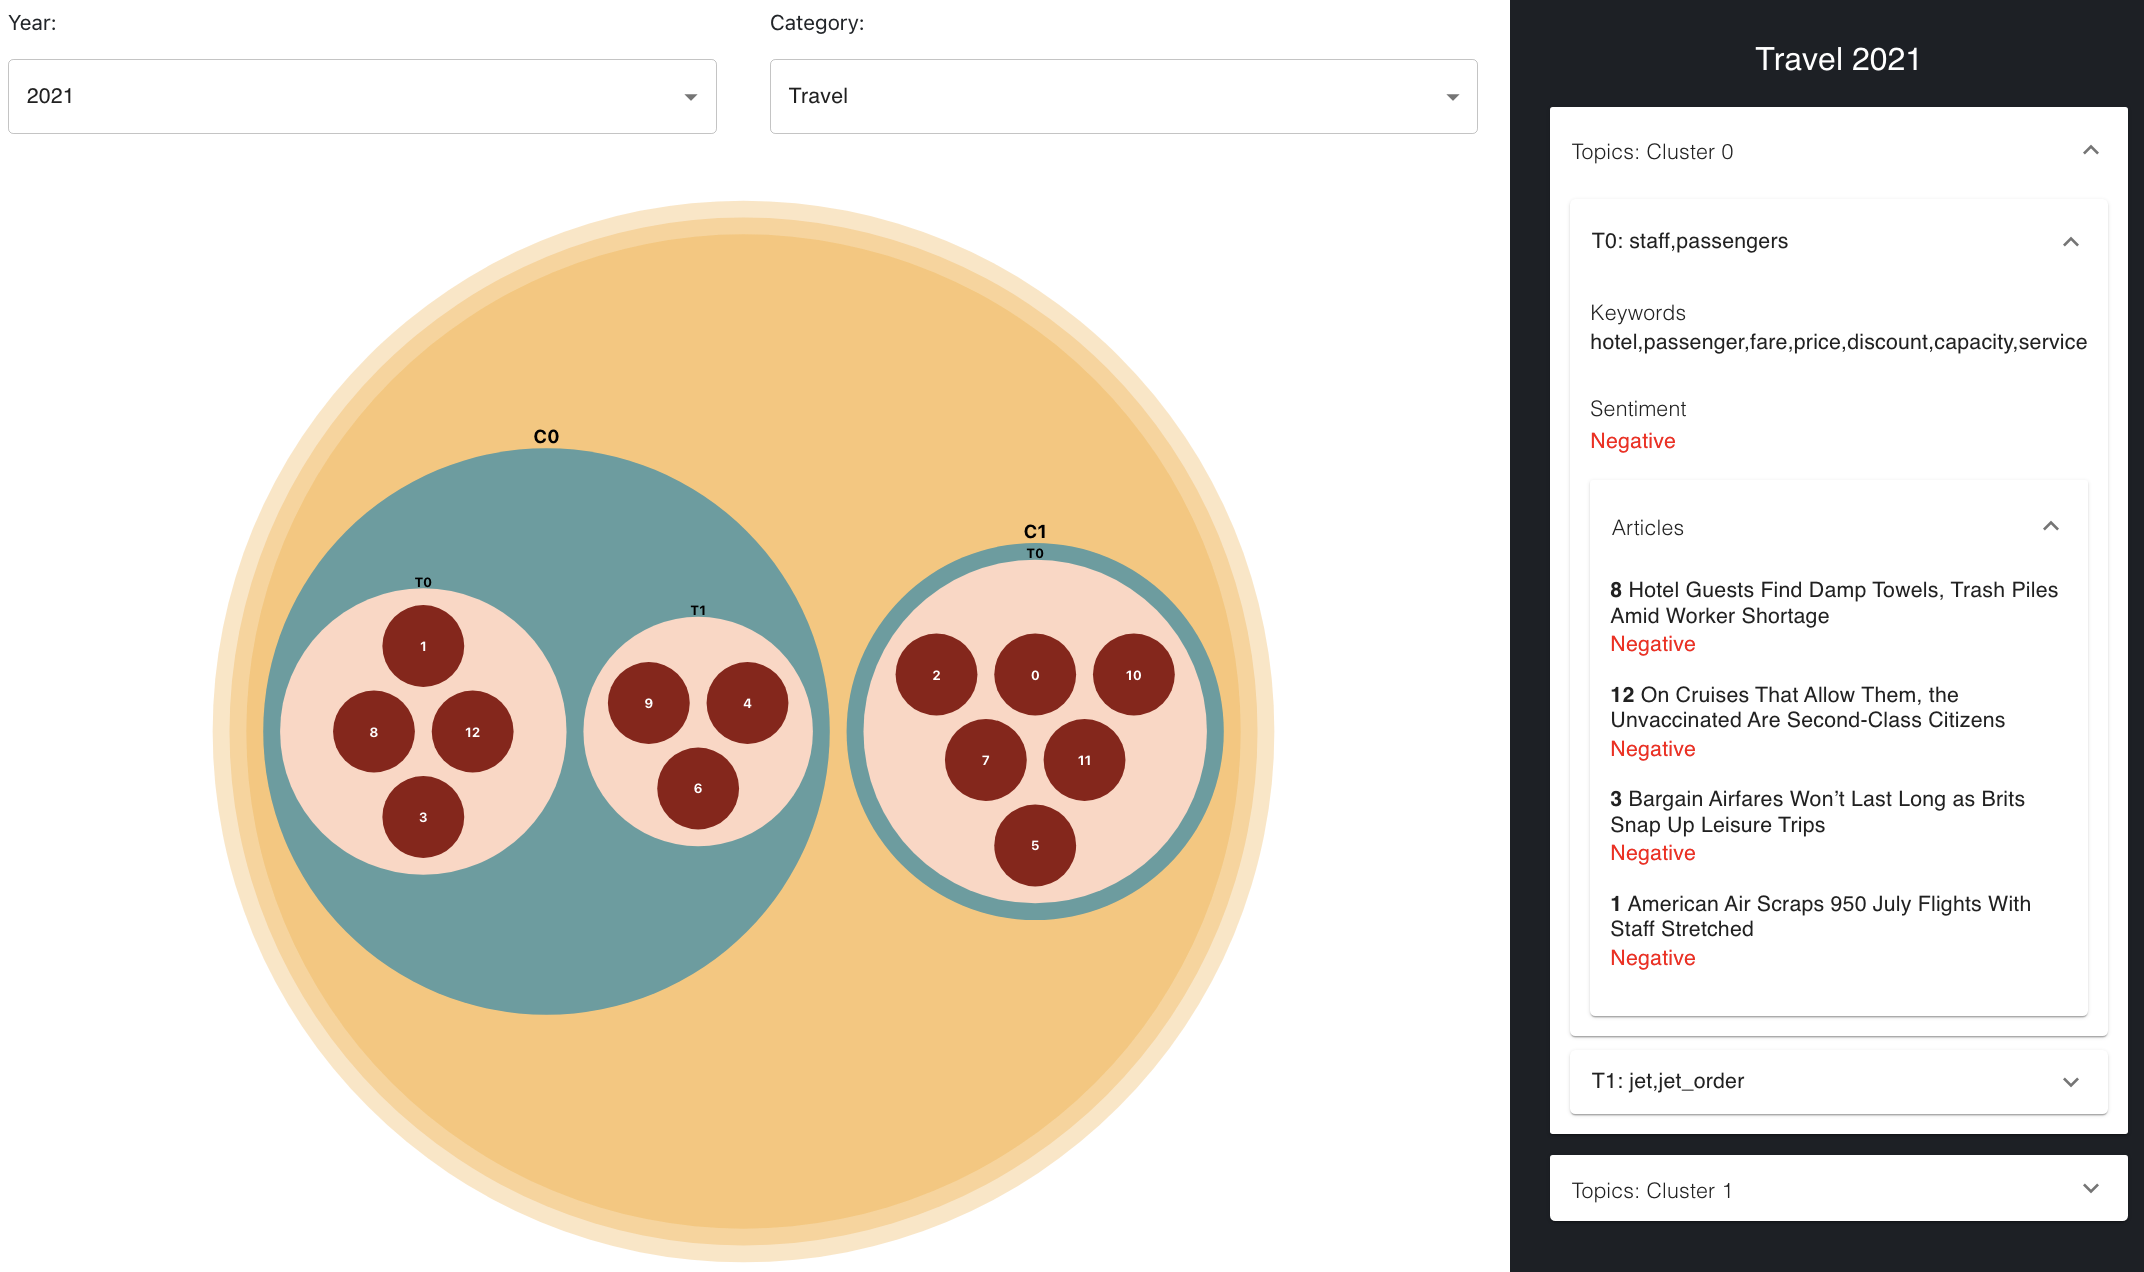
\includegraphics[width=0.85\linewidth]{images/travel2021_topics_cropped.png}
  \caption{}
  \label{fig:topics_travel2021}
\end{figure}
The aim of the was to derive semantic clusters from the article corpus for each Year-Category group and apply topic modelling from on these clusters to obtain topics and determine the articles belonging to these topics. This is shown in \Crefrange{fig:topics_travel2021}{fig:topics2_travel2021}. 

\Cref{fig:topics_travel2021} displays the `cluster-topic' graph for `Travel2021' which has 2 semantic clusters C0 and C1, with 2 and 1 topics respectively. This particular input group contained limited data and is used as an example for ease of understanding \hl{(See Appendix ???? for additional `cluster-topic' graphs for other input groups)}. We can see that one of the topics (T0) in Cluster 0 (C0) has the inferred topic name as `staff, passengers' with the topic keywords: `hotel', `passenger', `fare', `price', `discount', `capacity' and `service'. The articles within this topic (numbered 1,3,8,12) are all talk about passengers (`Hotel Guests' in article 8, `cruise' passengers in article 12, `British' passengers in article 3) and staff (`worker shortage' in article 8 and `staff stretched' in article 1). The keywords are also indicative of the general theme of the articles in the topic. All the articles in this topic are have `negative' sentiment as they generally focus on airlines struggling with poor service due to worker shortage, resulting in a `negative' average sentiment for the topic.

It is apparent that the semantic cluster C0 focuses on airlines and planes with T0 focusing on struggles with staff and passenger service and T1 on the new jet orders. This gives confidence in the engine to extract meaningful topics for the article corpus for a given semantic cluster. 

\begin{figure}[H]
  \centering
  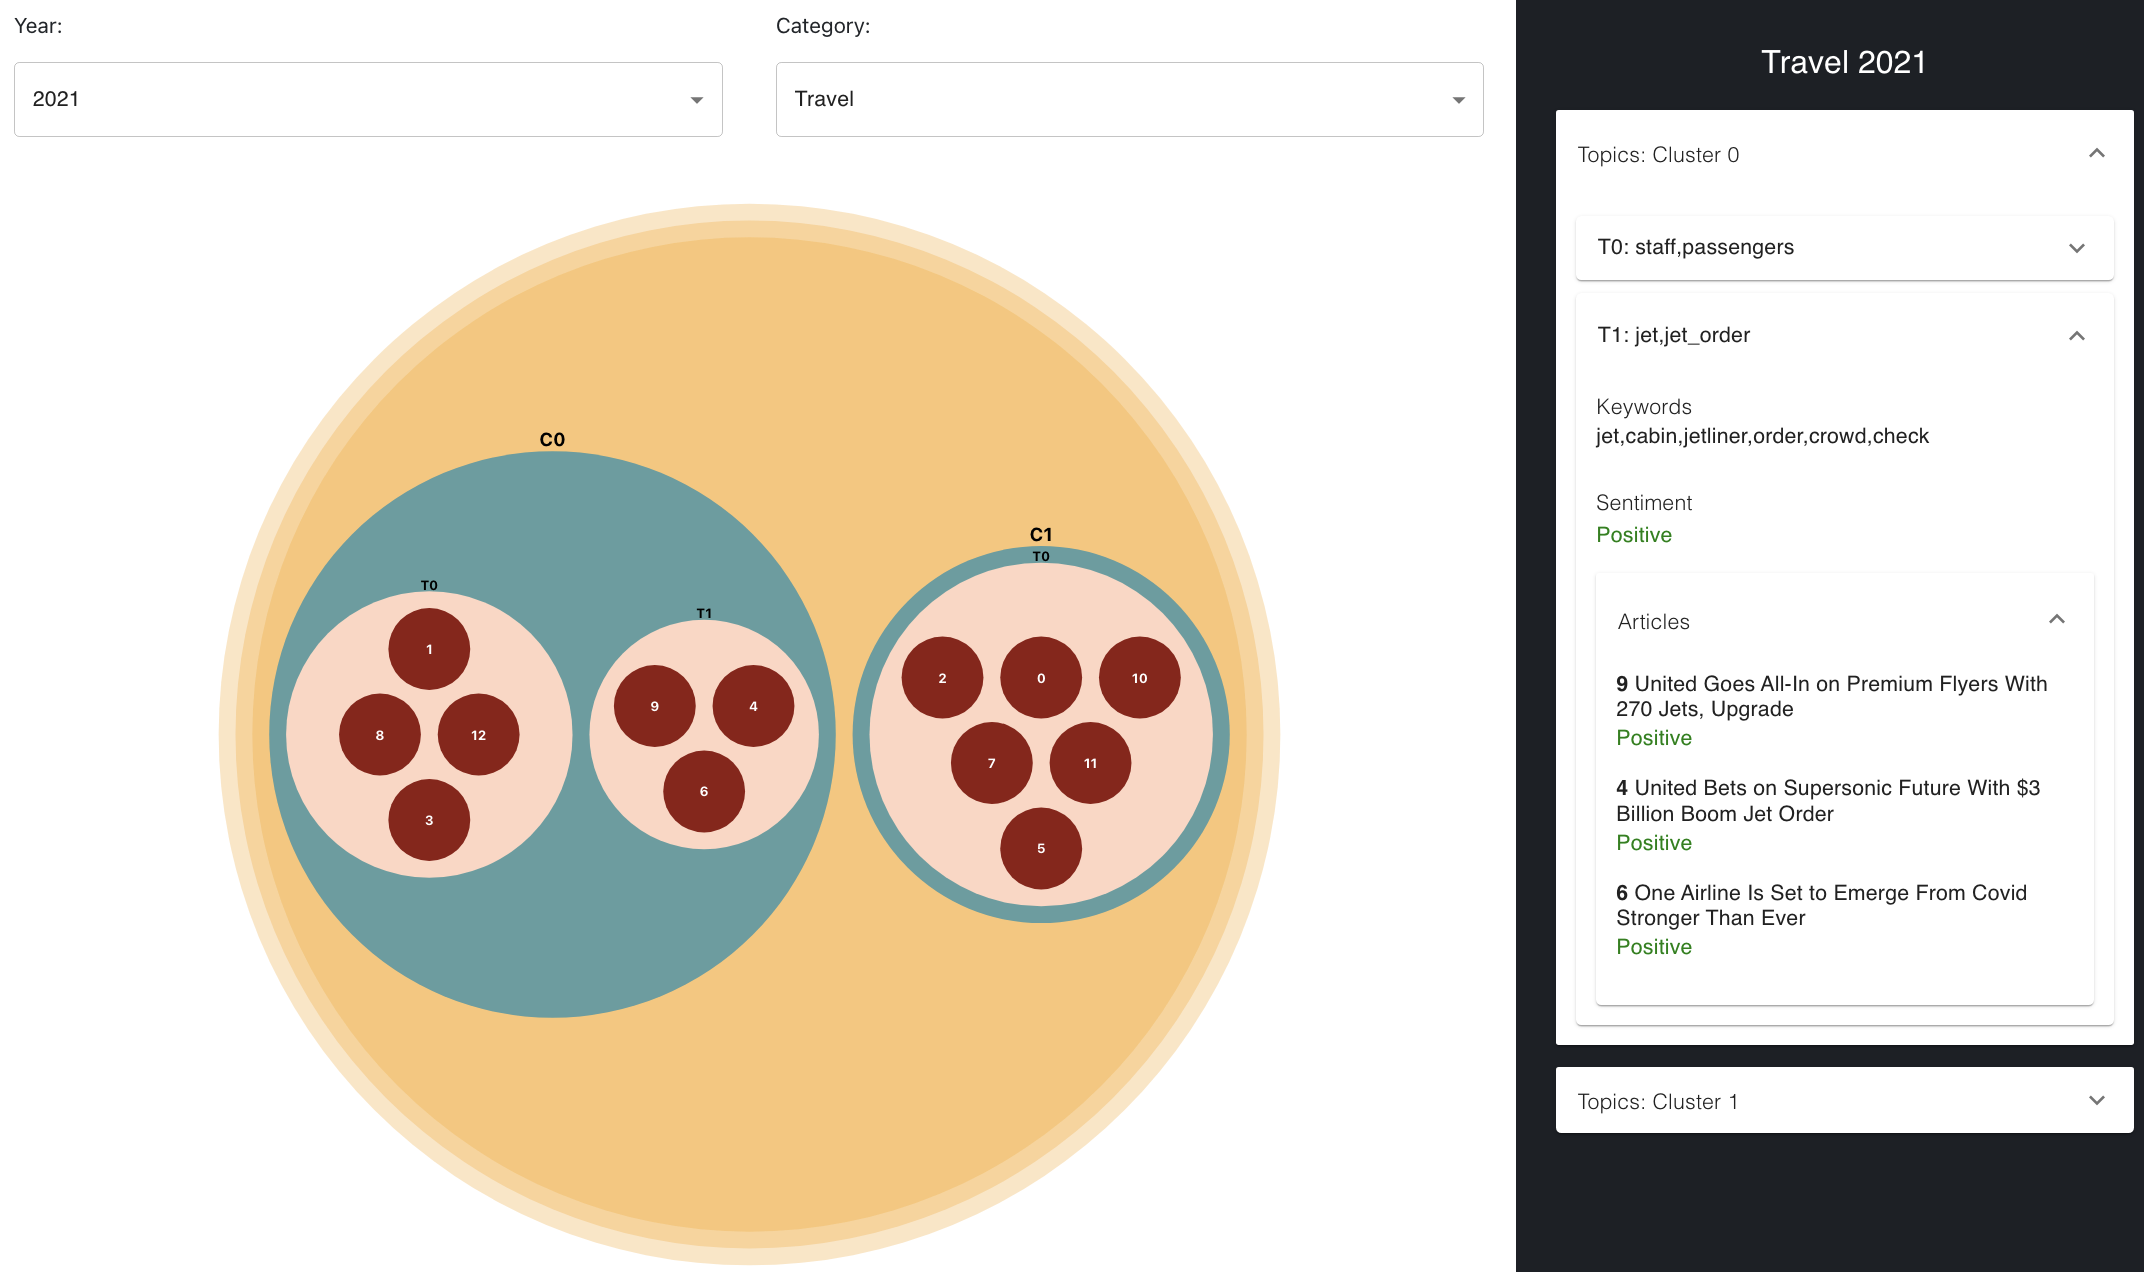
\includegraphics[width=0.95\linewidth]{images/travel2021_topics_1b.png}
  \caption{}
  \label{fig:topics1b_travel2021}
\end{figure}

\Cref{fig:topics1b_travel2021}, on the other hand, shows the other topic (T1) for the in the same semantic cluster (C0) with the inferred topic name as `jet, jet\_order' with the topic keywords: `jet', `cabin', `order', `jetliner', `crowd' and `check'. This topic differs from the previous topic as this focuses the positive developments made by airlines by investing into new planes and jets. All articles in this topic (numbered 9,4,6) have a `positive' sentiment resulting in overall average `positive' sentiment for this topic.


% topic keywords as `country', `tax, `arrival, `state', `reopening' and `tourist'.
\begin{figure}[H]
  \centering
  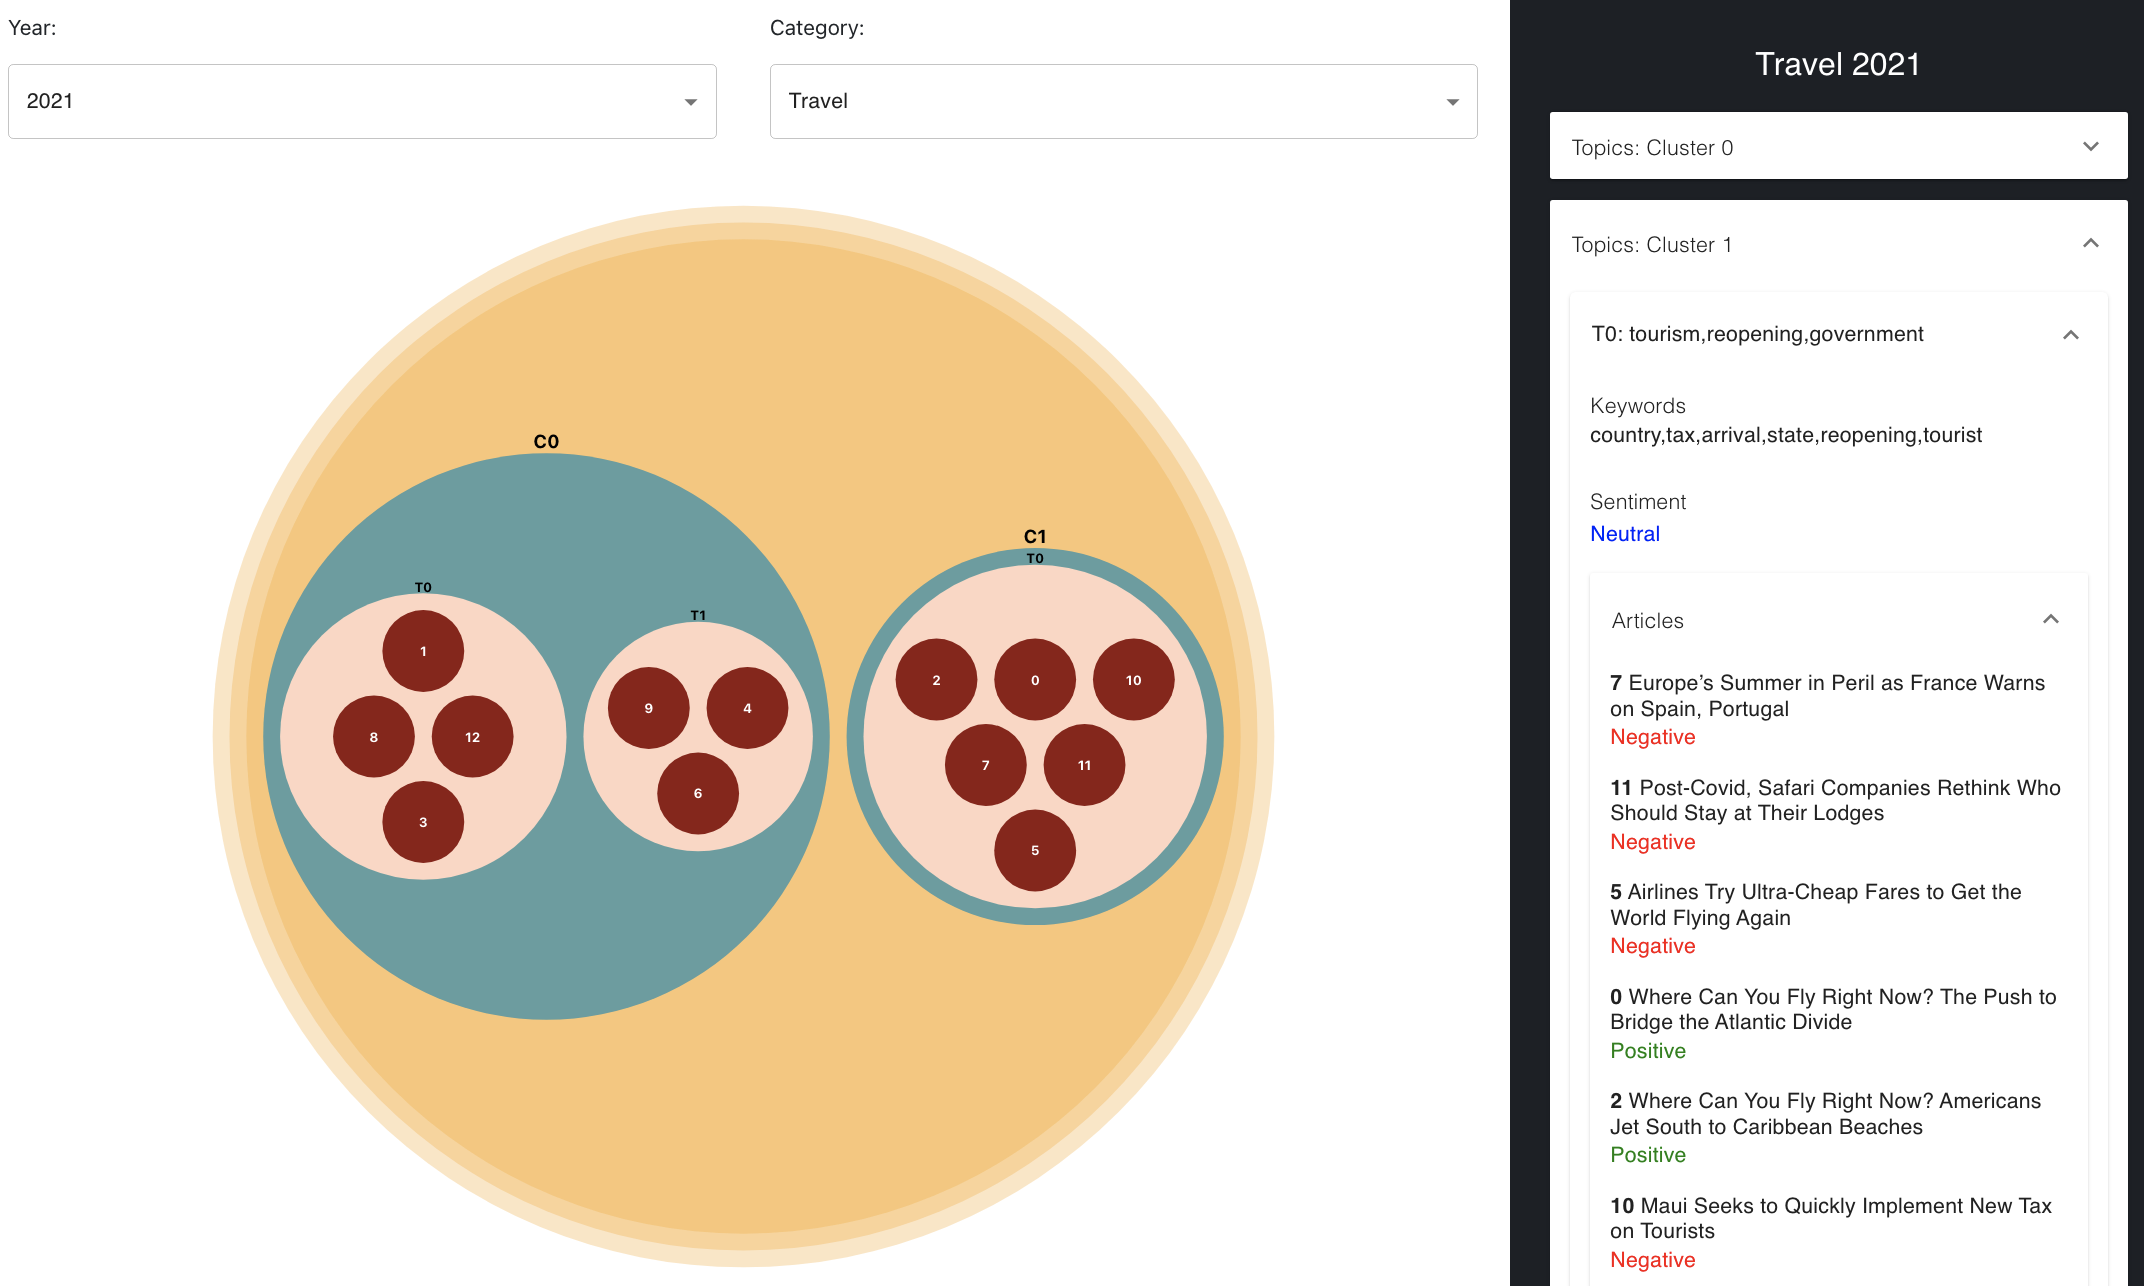
\includegraphics[width=0.95\linewidth]{images/travel2021_topics_2.png}
  \caption{}
  \label{fig:topics2_travel2021}
\end{figure}

\Cref{fig:topics2_travel2021} displays the information about the semantic cluster (C1) which has one topic with the inferred topic name `tourism, reopening, government' and keywords: `country', `tax', `arrival', `state', `reopening' and `tourist'. Unlike Cluster 0 (C0) this cluster (and topic) focuses on the tourism. We can see the divided approach in the articles which talk about implementing tourist taxes (article 10) and screening guests post-Covid (article 11) as well as airlines adopting cheaper fares and pushing travel (articles 0,2 and 5). This divided approach in post-Covid travel is reflected in the sentiments of these articles, resulting in a `Neutral' average sentiment.

Therefore, based on the \Crefrange{fig:topics_travel2021}{fig:topics2_travel2021}, we get confidence in the Topic Extraction Engine's semantic clustering, as we can see the different clusters extracted (C0: airlines and C1:tourism) and the distinct topics in these clusters, which provide an insight into the corresponding articles contributing to these topics as well as the associated sentiment regarding that topic. 

\subsection*{Limitations}
\todonum[inline]{Topic Engine: Write about limitations}